\chapter{Literature Review}
\label{sec:lit}

This chapter reviews the work that has already been done in both the
fields of garbage collection in Section \ref{sec:lit-gc}, and
algorithm verification in Section \ref{sec:lit-verification}, and then
considers in more detail some instances of verified collectors in
Section \ref{sec:lit-verifiedgc}.

The review is largely restricted to stop-the-world, non-concurrent,
non-hybrid\footnote{A garbage collector which just uses one method to
  collect the heap, such as mark-sweep, rather than combining multiple
  methods} collectors, as the project only directly involved such
simple collectors, as considering more complex situations would
significantly complicate the work. A brief mention is given to
generational collectors, which are arguably hybrid, but they are
not considered further.

Understanding the dissertation will require some understanding of
mark-sweep and copying collectors, Hoare logic, and array
reasoning. Other information provided in this review should be
considered as additional background information to give the reader
some greater appreciation of the field, but is not essential.

\section{Garbage Collection}
\label{sec:lit-gc}

Garbage collection is the process of automatically reclaiming unneeded
allocated memory from a program\cite{McCarthy60}. In languages with
manual memory management, such as C, a programmer can allocate new
memory with \texttt{malloc}, but then must remember to release it with
\texttt{free}\cite{KandR}. If this is not done, a memory leak occurs,
and the program may gradually consume more and more
memory\cite{Barach82}.

In a garbage collected language, however, the programmer can allocate
new memory, but typically cannot (and does not need to) explicitly
deallocate it. Instead, some runtime system determines when cells no
longer needed, typically by determining if they can be reached by
following pointers from the roots---the set of variables in scope---or
not.

We can divide most garbage collection algorithms into four camps:
reference counting, mark-sweep, copying, and
mark-compact\cite{GarbageCollection}. Each is suited to different
use-cases, and the choice of which to use is often determined by the
behaviour of the particular system in which they will be used.

Throughout this section, a visual example shall be used to aid
understanding. Figure \ref{fig:lit-gc-before} shows a heap before
garbage collection, and for each collector the same heap after
collection shall be shown. Green cells are those pointed to by the
roots (where pale green indicates those only pointed to indirectly:
the reachable cells), red are garbage, and white are free.

\begin{figure}[t]
  \centering
  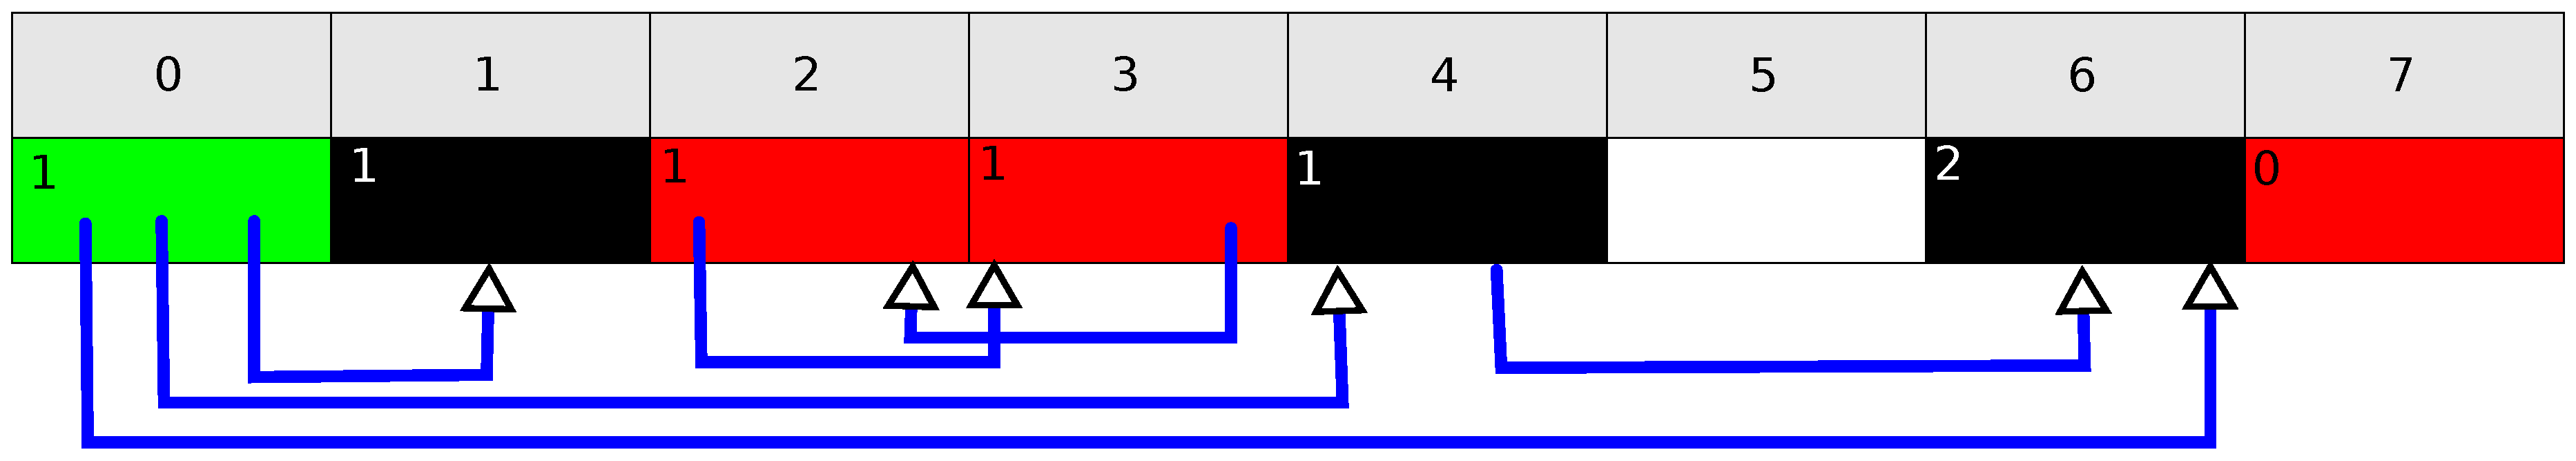
\includegraphics[width=\textwidth]{lit-gc-before}
  \captionsetup{format=default}
  \caption{Heap with garbage}
  \label{fig:lit-gc-before}
\end{figure}

\subsection{Reference Counting}
\label{sec:lit-gc-refcount}

\begin{figure}[t]
  \centering
  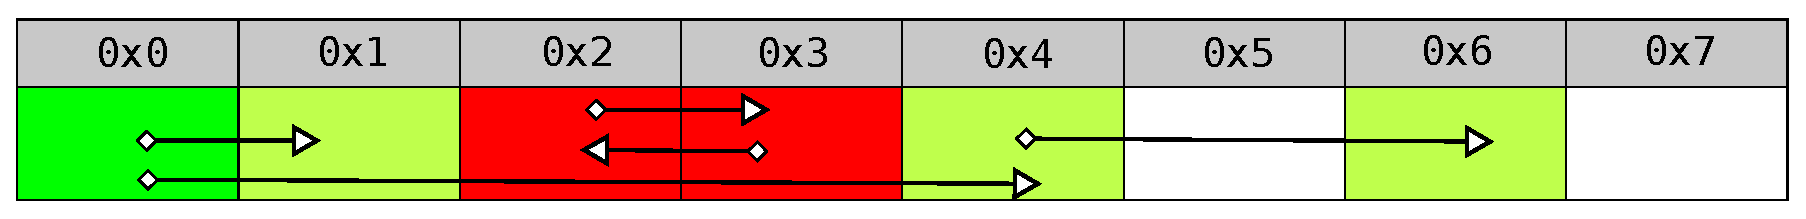
\includegraphics[width=\textwidth]{lit-gc-refcount}
  \caption{Heap after reference counting}
  \label{fig:lit-gc-refcount}
\end{figure}

Reference counting is a very simple scheme where each cell contains a
\textit{reference count}, some integer field which keeps track of the
number of references to the cell. In the most basic form of the
algorithm, the compiler maintains a write barrier, which increments
and decrements the count immediately as references are created or
destroyed. Furthermore, as soon as the count reaches zero, the cell is
deallocated\cite{Collins60}.

This strategy seems good, as it distributes the load of memory
management throughout the computation, however it results in the
problem of unbounded time taken to free a cell, as freeing it may
cause other things to be freed, and so on\cite{GarbageCollection}.
This problem can be offset by pushing to a free list, rather than
doing the recursive free, or by deferring the reference counting. The
Deutsch--Bobrow algorithm is an example of this kind, where reference
count adjustments are stored in a transaction file, which is routinely
processed to adjust the state of the entire system\cite{Deutsch76}.

A fatal flaw, alas, with reference counting is that it cannot reclaim
self-referential structures, as shown in the example, even if they are
garbage\cite{McBeth63}. Some systems make use of \textit{weak
  references}---references which do not cause the count to be
modified---to offset this\cite{Brown95}. However, this places a burden
on the programmer and so loses some of the convenience of the system.

\subsection{Mark-Sweep}
\label{sec:lit-gc-marksweep}

\begin{figure}[t]
  \centering
  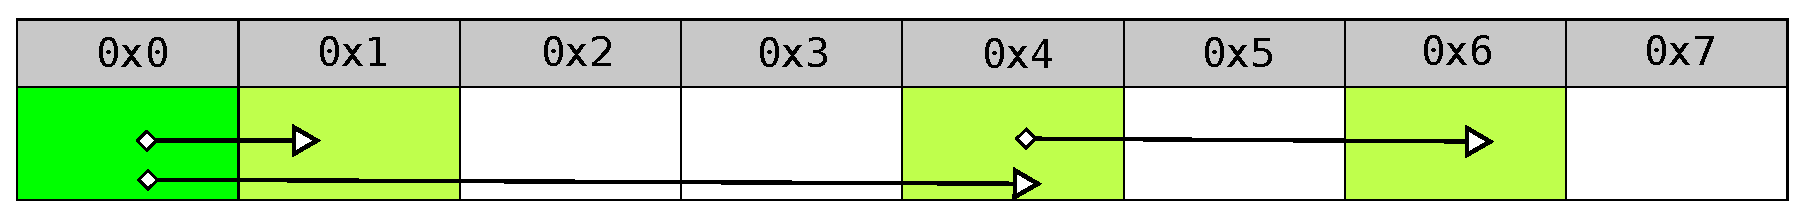
\includegraphics[width=\textwidth]{lit-gc-marksweep}
  \captionsetup{format=default}
  \caption{Heap after mark-sweep collection}
  \label{fig:lit-gc-marksweep}
\end{figure}

The mark-sweep method was invented for the early Lisp
systems\cite{McCarthy60}, and it functions by giving every cell a
\textit{mark bit}, which is initially unset. Upon running out of
memory, all cells reachable from the roots are marked (this can be
done recursively quite simply), and then all cells in the heap are
examined: those which are unmarked are freed, and those which are
marked are unmarked, ready for the next
collection\cite{GarbageCollection}.

Compared to reference counting, mark-sweep is a very different beast:
it handles cycles easily and there is no overhead on pointer
operations. It does, however, halt the computation\footnote{Sometimes
  called a stop-the-world collector} in order to perform a
collection\cite{GarbageCollection}. Furthermore, garbage collection
becomes more frequent as heap residency increases\cite{McCarthy60},
and the blocking time is proportional to the size of the
heap\cite{Appel87}.

These problems can be offset somewhat by interleaving the sweeping
with the mutator: the garbage collected program, so called because it
mutates the heap\cite{Dijkstra78}. Hughes's lazy sweep
algorithm\cite{Hughes82} does this by performing a fixed amount of
sweeping at each allocation, and so the only long garbage collection
pause happens when the heap needs to be marked.

\subsection{Copying}
\label{sec:lit-gc-copying}

\begin{figure}[t]
  \centering
  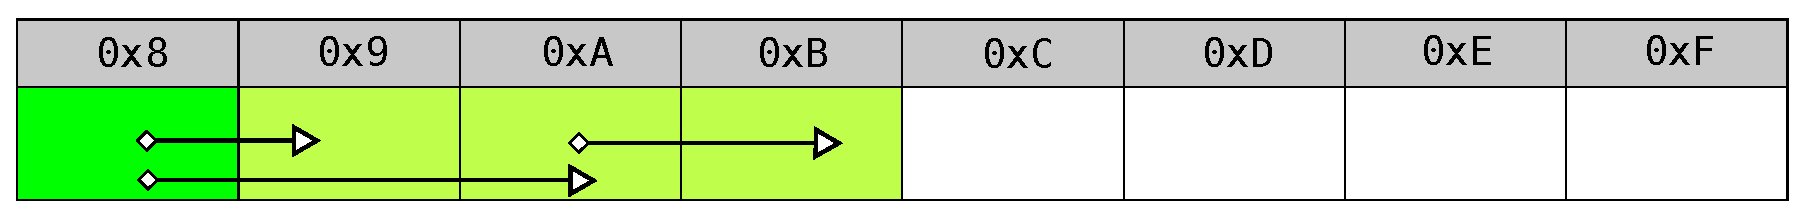
\includegraphics[width=\textwidth]{lit-gc-copying}
  \caption{Heap after copying collection}
  \label{fig:lit-gc-copying}
\end{figure}

Copying collectors divide the heap into two \textit{semispaces}, where
allocation is only done in one of them at a time. In garbage
collection, all live cell are copied to the other semispace (in the
example this has been shown by shifting the addresses up by 8), and
the roles of the semispaces are swapped\cite{Fenichel69}. Unlike
mark-sweep collectors, the pause time of a copying collector is
proportional only to the number of live cells\cite{Appel87}.

Copying collectors have become fairly popular due to the low cost of
allocation and reduction of fragmentation, however they have a space
cost of a half of the heap space\cite{GarbageCollection}.

\subsection{Mark-Compact}
\label{sec:lit-gc-markcompact}

\begin{figure}[t]
  \centering
  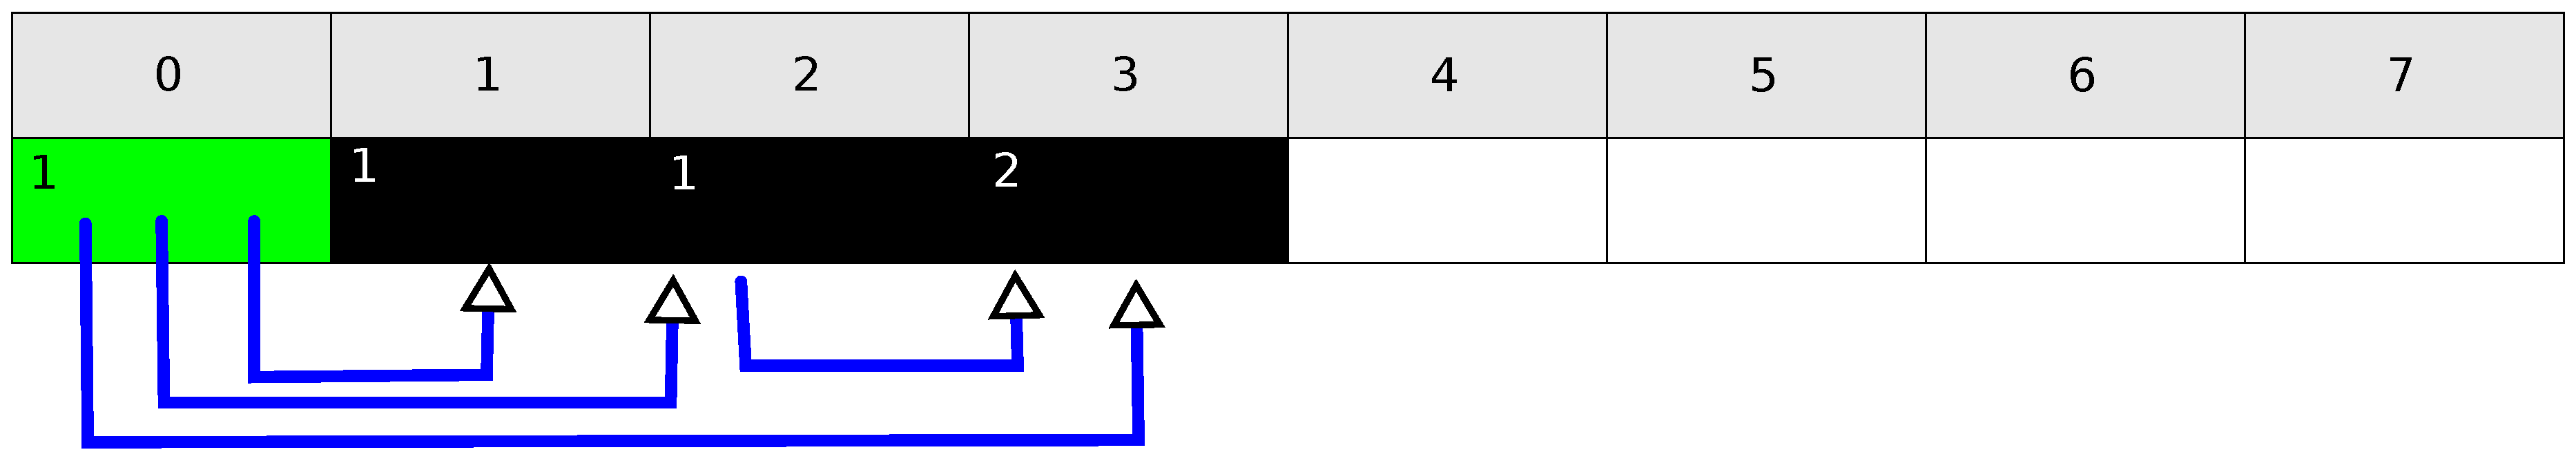
\includegraphics[width=\textwidth]{lit-gc-markcompact}
  \caption{Heap after mark-compact collection}
  \label{fig:lit-gc-markcompact}
\end{figure}

Heap fragmentation can be a great problem: there may be more than
enough space to allocate something, but not enough contiguous space to
do so. Furthermore, high fragmentation can increase the rate of page
faults and cache misses, reducing the performance of the
mutator\cite{Zorn90}.

Thus, we come to the mark-compact collectors. These first mark the
live portion of the heap, and then copy marked cells over garbage
ones, moving everything towards one end of the heap in order to remove
fragmentation\cite{GarbageCollection}. There are three ways of
performing this compacting: cells can be moved without regard for
their original order; cells which point to each other can be placed
next to each other; and cells can simply `slide' towards one end of the
heap\cite{Cohen81}.

Unfortunately, these collectors require multiple traversals over the
heap, and so are potentially even slower than mark-sweep
collectors\cite{GarbageCollection}.

\subsection{Hybrid Collectors}
\label{sec:lit-gc-hybrid}

Sometimes any one of these standard algorithms is not quite good
enough for a particular problem, and a better collector can be formed
by combining them. For example, reference counting could be combined
with periodic copying, in order to reclaim cyclic structures and
reduce fragmentation. Immix\cite{Blackburn08} is a hybrid mark-region
(memory is divided into large regions, inside which allocation occurs)
and copying collector.

A common type of hybrid collector is a generational garbage collector,
which is composed of an incremental, typically copying, stage, and a
whole-heap collection stage.

\subsubsection{Generational Collectors}
\label{sec:lit-gc-hybrid-generational}

Generational garbage collectors are a type of hybrid collector: the
heap is divided into a number of \textit{generations}, where each
generation holds progressively older cells. This technique is based on
empirical observations of cell lifetimes resulting in the generational
hypothesis: young objects tend to die quickly, whereas old objects
tend to stick around\cite{Ungar84}.

Allocation happens in the youngest generation, and when that fills up
a \textit{minor collection} is started. The generation is garbage
collected, and old enough cells get copied to the next
generation\cite{Ungar84}. In the simplest case, all live cells at the
time of a minor collection get promoted. If the entire heap is full, a
\textit{major collection} is started, which uses some other garbage
collection algorithm\cite{GarbageCollection}.

Generational garbage collection tends to perform well for languages
where old-to-young pointers are rare\cite{Appel89}, such as most
functional languages, and so has become fairly popular amongst
implementers of such
languages\cite{Rojemo95}\cite{Sansom93}\cite{Seward92}.

\section{Algorithm Verification}
\label{sec:lit-verification}

Algorithm verification (or software verification) is the process of
constructing a mathematical proof that an algorithm behaves as we
expect it to\cite{Floyd67}. In the case of software, we may prove the
actual code implements the specification; in the case of an algorithm,
we may be satisfied with merely proving that it satisfies various
properties, such as termination.

We need verification because testing can never show that there are no
bugs, it can only show that there have been no bugs found yet, to
quote Dijkstra, ``testing shows the presence, not the absence of
bugs''\cite{Buxton70}. A formal proof provides a much stronger
guarantee than can be obtained by testing or inspection alone.

There are two methods of verification: constructing the algorithm and
then proving things about it, and constructing a proof and then
extracting an algorithm out of it.

\subsection{Verification by Embedding}
\label{sec:lit-verification-embedding}

This is arguably the more difficult method of verification, as it
consists of taking a fairly low-level implementation, often at the
level of code, and a very high-level specification and proving things
about the relationship between the two.

To begin with, the implementation must be formalised using some logic
such as Hoare logic\cite{Hoare69}, which defines the semantics for a
very simple imperative language, or separation logic\cite{Reynolds02},
which is similar to Hoare logic but adds axioms for reasoning about
the stack and heap.

Once formalised, the axioms of the logic can be used to deduce
propositions about the implementation. Deduction can be, to some
extent, automated using proof assistants, but in general this is
undecidable.

\begin{example}[Finding the index of the minimal element of a nonempty
  sequence of integers]
  \label{exmpl:lit-embedding}
  As an example of verification by embedding, consider the following
  short program, to find the index of the minimal element in a
  sequence of integers:

\begin{verbatim}
i := 1;
j := 1;
while j < len xs do
    if xs[j] < xs[i] then
        i := j
    else
        skip
    j := j + 1
\end{verbatim}

  We shall call this program $P$, and $xs$ is some sequence of
  integers. For (partial) correctness of this program, we want to
  establish (using Hoare triples) $\htriple{\len xs > 0}{P}{xs[i] =
    \min xs}$. A Hoare triple $\htriple{P}{S}{Q}$ states that if the
  assertion $P$ holds before executing a statement $S$, then the
  assertion $Q$ holds afterwards.

  A condensed proof tree is presented in Figure
  \ref{fig:exmpl:lit-embedding-tree}, with further proofs in Figures
  \ref{fig:exmpl:lit-embedding-sequencing} and
  \ref{fig:exmpl:lit-embedding-loop}.

  \begin{figure}[t]
    \centering
    \begin{prooftree}
      \AxiomC{$\htriple{I[1/j][0/i]}{i := 0; j := 1}{I}$}
      \AxiomC{$I[1/j][0/i] \iff L$}
      \BinaryInfC{$\htriple{L}{i := 0; j := 1}{I}$}

      \AxiomC{$\htriple{I \land R(j)}{if \ldots}{S}$}
      \AxiomC{$\htriple{S}{j := j + 1}{I}$}
      \BinaryInfC{$\htriple{R(j) \land I}{if \ldots; j := j + 1}{I}$}

      \BinaryInfC{$\htriple{\len xs > 0}{P}{xs[i] = \min xs}$}
    \end{prooftree}
    \caption{Proof tree for the embedding example}
    \label{fig:exmpl:lit-embedding-tree}
  \end{figure}

  Some definitions used in the proof trees are as follows,

  \begin{align*}
    R(x) &\equiv x < \len xs\\
    C    &\equiv xs[i] = \min xs\\
    C_{T} & \equiv I \land R(j) \land xs[j] < xs[i]\\
    C_{F} & \equiv I \land R(j) \land \lnot(xs[j] < xs[i])\\
    L    & \equiv \len xs > 0\\
    I    & \equiv xs[i] = \min \{xs[a]~|~0 \leq a < j\}\\
    S    & \equiv I \land xs[i] \leq xs[j] \land R(j)
  \end{align*}

  A full proof is omitted here as it is not essential to appreciate
  the example.
\end{example}

This approach is good to take if the property to be proven is more
easily expressed by code than by proof. For example, a garbage
collector may move things around in memory. Producing a constructive
proof (as is used in extraction) that this is soluble and then
plucking out the desired algorithm may be more difficult than
implementing the algorithm, and then showing that is satisfies an
appropriate invariant.

\subsubsection{Preconditions and Postconditions}
\label{sec:lit-verification-embedding-conditions}

A precondition is some assertion which must hold before executing some
code, and a postcondition is some assertion which must hold
afterwards\cite{Hoare69}, Hoare triples express this.

In the case of languages with formally specified semantics, we must be
able to derive the postcondition from the precondition and the
code. One approach is establishing the desired postcondition (the
result of executing the code), and then working from end to beginning,
in order to figure out what the necessary preconditions are, this is
known as backwards chaining\cite{Russell05}. If both the precondition
and postcondition of some sequence of code are known, then the proof
can progress inwards from both ends, meeting in the middle. If the two
proof efforts cannot be unified, then there is a flaw in the code.

Common to many proof systems is the ability to strengthen
preconditions and weaken postconditions\cite{Hoare69}, this is legal
because if precondition $P'$ implies $P$, then by using the
precondition $P'$ instead of $P$, we know that $P$ is guaranteed to
hold. Similarly, if postcondition $Q$ implies $Q'$, then we know that
$Q'$ is guaranteed to hold. The ability to do this is expressed by the
Hoare consequence rule:

\begin{prooftree}
  \AxiomC{$P' \implies P$}
  \AxiomC{$\htriple{P}{S}{Q}$}
  \AxiomC{$Q \implies Q'$}
  \TrinaryInfC{$\htriple{P'}{S}{Q'}$}
\end{prooftree}

This allows localised proofs to be used in a larger proof, and so
facilitates modularity by allowing proofs of some components of a
program to be considered independently, and then combined later on.

\subsubsection{Axiomatic Semantics}
\label{sec:lit-verification-embedding-axioms}

\begin{figure}[t]
  \centering
  \begin{prooftree}
      \AxiomC{$\htriple{I[1/j][0/i]}{i := 0}{I[0/j]}$}
      \AxiomC{$\htriple{I[1/j]}{j := 1}{I}$}
      \BinaryInfC{$\htriple{I[1/j][0/i]}{i := 0; j := 1}{I}$}
      \AxiomC{$I[1/j][0/i] \iff L$}
      \BinaryInfC{$\htriple{L}{i := 0; j := 1}{I}$}
  \end{prooftree}
  \caption{Sequencing of statements in Hoare logic}
  \label{fig:exmpl:lit-embedding-sequencing}
\end{figure}

Axiomatic semantics allow us to reason about programs by providing
tools to reason about the effect of program statements on program
state\cite{Hoare69}. These are closely connected with Hoare logic. A
simple example is the Hoare rule for composition:

\begin{prooftree}
  \AxiomC{$\htriple{P}{S}{Q}$}
  \AxiomC{$\htriple{Q}{T}{R}$}
  \BinaryInfC{$\htriple{P}{S; T}{R}$}
\end{prooftree}

This states that if we have two statements, $S$ and $T$, where the
postcondition of $S$ is the precondition of $T$, then we can combine
the two into the compound statement $S;T$\cite{Hoare69}. In Hoare
logic, there are rules for assignment, \textit{skip} (the statement
which does nothing), while loops, conditional statements, and
consequence.

In general, axiomatic semantics specify how the post-state of a
statement refers to the pre-state. They should be consistent but, as
a consequence of G{\"o}del's incompleteness theorems, this cannot
necessarily be proven.

Given these rules, we can very easily deconstruct a program into a
proof tree showing how all of the assertions are related, which is
often a very good starting point for then constructing a specific
proof for the property we wish to establish.

\subsubsection{Loop Invariants}
\label{sec:lit-verification-embedding-invariants}

\begin{figure}[t]
  \centering
  \begin{prooftree}
    \AxiomC{$C_{T} \implies S[j/i]$}
    \UnaryInfC{$\htriple{C_{T}}{i := j}{S}$}

    \AxiomC{$C_{F} \iff S$}
    \AxiomC{$\htriple{C_{F}}{skip}{C_{F}}$}
    \BinaryInfC{$\htriple{C_{F}}{skip}{S}$}
    \BinaryInfC{$\htriple{I \land R(j)}{if \ldots}{S}$}

    \AxiomC{$S \implies I[j + 1/j]$}
    \AxiomC{$S \implies I$}
    \BinaryInfC{$\htriple{S}{j := j + 1}{I}$}

    \BinaryInfC{$\htriple{R(j) \land I}{if \ldots; j := j + 1}{I}$}
    \UnaryInfC{$\htriple{I}{while \ldots}{\lnot R(j) \land I}$}
  \end{prooftree}
  \caption{Loop invariants in Hoare logic}
  \label{fig:exmpl:lit-embedding-loop}
\end{figure}

Proofs of programs involving loops rely on finding a loop invariant:
some property which does not change over time as the loop is
executed\cite{Hoare69}. This is expressed in Hoare logic with the
while rule:

\begin{prooftree}
  \AxiomC{$\htriple{I \land B}{S}{I}$}
  \UnaryInfC{$\htriple{I}{while B do S}{\lnot B \land I}$}
\end{prooftree}

$I$ is the loop invariant, $B$ is the loop condition, and $S$ is the
statement that is the loop body. The premise is read ``if the
proposition $I \land B$ holds, then after doing S once, the
proposition $I$ holds,'' and the consequence is read ``if the
proposition $I$ holds, then after doing the loop \textit{while B do
  S}, the proposition $\lnot B \land I$ holds''. Thus, we can see that
$I$ is invariant.

The only information we can extract from a loop, at least under Hoare
logic, is $\lnot B$, which doesn't seem very useful. The loop may be
doing something very complicated, but it seems we can only extract a
very small bit of information about it. The difficulty, then, lies in
finding a loop invariant that, when combined with $\lnot B$, yields
the result we want.

\subsection{Verification by Extraction}
\label{sec:lit-verification-extraction}

The other approach is to gradually work downwards from the high-level
specification to a constructive proof, which can then be turned into
an implementation. Gradually turning a specification into an
implementation in this way is called refinement. A special case of
refinement is when the specification is already in the form of a
constructive proof, in which case we can extract the implicit program
from it, this is called extraction.

We start out by formalising the specification in some logic, such as Z
or HOL, and then construct a slightly lower-level specification and
prove that it is a correct refinement of the higher-level one by
reasoning about the pre- and post-conditions of each abstract
operation\cite{Woodcock96}. Whilst it may take many refinement steps
to get actual code out of this process, each proof is between two very
similar specifications, and so may be easier than the verification by
embedding method. Proof assistants may be more useful here than in
verification by embedding, but here the difficulty lies in finding the
appropriate invariant to relate the two steps\cite{Woodcock96}.

Furthermore, there are often multiple choices of refinement step
available, and so the first few steps can be reused to construct
different algorithms, simply by making different choices at the lower
levels\cite{Myreen10}.

\begin{example}[Finding the index of the minimal element of a nonempty
  sequence of integers]
\label{exmpl:lit-extraction}
For all nonempty sequences of integers, there exists an index of a
minimum element.

\[\forall n \in \mathbb N,\
\forall x_{1}, x_{2}, \ldots x_{n} \in \mathbb Z,\ 
\exists 1 \leq m \leq n,\ 
\forall 1 \leq i \leq n,\ 
x_{m} \leq x_{i}\]

Proof is by induction.

\begin{description}
  \item[Base case (n=1)] $m = 1$ is a witness, by reflexivity of
    $\leq$.

  \item[Inductive case (n=k+1)] Divide the sequence into its head
    and tail (the latter being of length $k$). Call the head $x$ and
    the tail $xs$, for simplicity. Solve the case for $xs$, and call
    the witness $m_{k}$.
    \begin{description}
      \item[If $x \leq xs_{m_k}$] Then $m = 1$ is a witness, by
        transitivity of $\leq$.

      \item[If $xs_{m_k} < x$] Then $m = m_{k} + 1$ is a witness, as
        $xs_{1}$ is actually as position 2 in the original sequence
        (it is all shifted right by one place).
    \end{description}
\end{description}

We can now, fairly directly, translate this proof into the following
Haskell program:

\begin{lstlisting}[language=haskell]
import Data.List (genericIndex)

f :: [Integer] -> Integer
f sequence = case sequence of
               [_] -> 1
               (x:xs) -> let mk = f xs
                         in if x <= genericIndex xs (mk - 1)
                            then 1
                            else 1 + mk
\end{lstlisting}

Even in such a short program, there are a couple of language-imposed
complications, due to the mismatch of types. Firstly, the
\texttt{genericIndex} function has to be used, as the list-indexing
operator \texttt{(!!)} takes the index as a machine word; and
secondly, the \texttt{mk} value has to be decremented when indexing,
as list indices in Haskell start from 0, not 1.

We can now apply semantics-preserving transformations to produce more
idiomatic code:

\begin{lstlisting}[language=haskell]
f :: [Integer] -> Integer
f (x:xs) | x <= genericIndex xs (mk - 1) = 1
         | otherwise = 1 + mk
         where mk = f xs
f _ = 1
\end{lstlisting}
\end{example}

This approach is good to take if the algorithm to be proven is quite
complex, and would be difficult to prove correct by itself, but where
the process of refining it from an initial specification may be
easier. For example, we could start out with a formalism for garbage
collection correctness, and then refine that until we produce an
actual collector.

\subsubsection{Constructive Proof}
\label{sec:lit-verification-extraction-constructive}

Often when proving that a problem is soluble, we do not care about how
an answer can be found, only that one exists, which can lead to very
concise existence proofs; when extracting a program directly from the
proof, however, we need to be able to show how to find the
answer. When refining from a specification, we start out with such an
abstract proof, and then gradually make it more constructive with each
step.

We can do this by using witnesses in our proof. A witness is a value
which shows a proposition to be correct. For example, $x = 2$ is a
witness for $\exists x \in \mathbb N, x > 1$. If we know how to find a
witness for everything we prove, then we know how to solve the
problem.

\subsubsection{Case Analysis}
\label{sec:lit-verification-extraction-cases}

Proofs often diverge into multiple cases to be shown. For example, an
inductive proof, covered in more detail in the next section, has a
base case and an inductive case. Only by proving both cases do we
prove the whole.

Given a constructive proof, we can translate a case analysis to a
switch statement, or conditional statement, in our program, and use
the witnesses for each case to construct the solution to the entire
switch.

\subsubsection{Induction, Recursion, and Iteration}
\label{sec:lit-verification-extraction-induction}

Proofs by induction require proving a base case, and then proving an
inductive case given the inductive hypothesis (being able to solve a
slightly smaller problem) holds, which naturally translates to the
programming methodology of reduce-and-conquer.

We can translate induction into iteration as follows:

\begin{enumerate}
  \item The base case is set up by the program at the beginning
  \item The inductive case is performed one step at a time in a while
    loop
\end{enumerate}

This is similar to the ladder-climbing analogy for induction: if you
can get on the first rung, then you can get to the top, simply by
going up one rung at a time.

We can translate induction into recursion similarly:

\begin{enumerate}
  \item The base case is the recursive base case
  \item The inductive case is the recursive case
\end{enumerate}

This, perhaps, is a more natural translation of induction, as it
directly illustrates the splitting up of the problem into a slightly
smaller one.

\subsubsection{Types}
\label{sec:lit-verification-extraction-types}

We must be careful to honour any non-obvious assumptions in the
proof. For example, if a proof requires a value to be a natural
number, then we cannot use machine words in our program, unless it can
also be proven that the natural numbers in question will always fit
into this range.

A famous example of a problem arising from this was in an
implementation of a binary search algorithm proven correct by
Bentley\cite{Bentley86}, which suffered from an integer overflow
problem. The proof assumed mathematical integers, but the
implementation did not provide this.

More generally, types in programming languages may not be identical to
types used in proofs, and we must be careful not to invalidate the
proof by getting the implementation types incorrect.

\subsubsection{Program Transformations}
\label{sec:lit-verification-extraction-transformation}

When we extract a program from a proof, the structure of the program
very closely mirrors that of the proof, as would be expected. However,
this may not be considered good style. We can apply arbitrary
transformations to the code of the extracted program, as long as these
transformations preserve the semantics.

\section{Verified Garbage Collection}
\label{sec:lit-verifiedgc}

Finally, we look at some examples of garbage collectors which have
been verified in different ways: a copying collector verified by
extraction, a different copying collector verified by embedding, and
finally a generic framework for verifying collectors and mutators.

\subsection{Reusable verification of a copying collector}
\label{sec:lit-verifiedgc-myreen}

Myreen\cite{Myreen10} has constructed a verified garbage collector
using the extraction method: correctness was formalised using the HOL4
theorem prover, was refined to produce an algorithm for correct
copying collectors, and was then refined further to the level of
verified machine code.

The collectors produced have been named L1, which is a specification
of copying garbage collection; L2, which is an implementation of L1 as
the transitive closure of a step relation; L3, which is a
deterministic implementation of L2 with more realistic memory
semantics; L4, which uses actual implementation types; and L5, which
is verified machine code. L5 is constructed by earlier work of Myreen,
on constructing a certifying compiler.

The initial collector is defined as a relation which restricts the
heap to live cells, and performs consistent renaming, \[x \gc y =
(\mathrm{filter}~x) \translate y\] and this specification is connected
to the lower-level L2 collector with an invariant, $\mathrm{inv}$
(where $x$ is a heap and $s$ and $t$ are root sets), \[\forall
x,~s,~t.\ \mathrm{inv}~x~s \land s \xrightarrow{step} t \implies
\mathrm{inv}~x~t\] which is presented as an 11-line HOL specification
in the paper.

Other than the obvious, the main contribution of Myreen is that his
proof is quite generic, as only the lowest level of refinement (L5)
makes use of a specific programming logic, and could be applied to many
different copying collectors, just by changing the specific refinement
steps taken.

\subsection{Local Reasoning about a Copying Garbage Collector}
\label{sec:lit-verifiedgc-birkedal}

Birkedal, Torp-Smith, and Reynolds\cite{Birkedal04} took a very
different approach to Myreen, they took an existing garbage collector
(Cheney's copying collector) and proved it correct, using a variant of
separation logic, in a Hoare-style proof, \[\htriple{(\exists y.\ e
  \mapsto y \land A) \land x = e'}{x := [e]}{e[e'/x] \mapsto x \land
  A[x/y]}\]

Similarly to Myreen, they defined correctness in terms of a heap
isomorphism modulo garbage cells, and in particular, that the
resultant heap has no garbage cells whatsoever.

The motivation of this paper is to be a stepping stone towards
programming logics which incorporate garbage collection, and so being
able to prove the correctness of the combination of a program and a
language runtime, which has thus far not been feasible.

This paper contributes to the field an extension of separation logic
with semantics for more types of assertion over finite sets, which is
used to express the isomorphism property of the algorithm. Needless to
say, this is an essential property of any garbage collector which
moves data around in the heap.

The major difference between these two verified garbage collectors is
that Myreen used extraction whereas Birkedal \textit{et al.} used
embedding. Thus, this proof cannot really be generalised to other
collectors, although the definition of correctness and logic developed
can, whereas Myreen's proofs are much more applicable to copying
collectors in general.

\subsection{A General Framework for Certifying Garbage Collectors and Their Mutators}
\label{sec:lit-verifying-mccreight}

McCreight, Shao, Lin, and Li\cite{McCreight07} produced a generic
method for certifying collectors and mutators independently, which is
very similar to the intended goals of this project. I unfortunately
only found this paper very late in the project (the latter half of
Spring term), after which the majority of the work had been done.

Their approach is to define an abstract interface between the
collector and mutator. The mutator works with an abstract heap,
whereas the collector works with the concrete heap, and the mapping
between the two is defined on a per-collector basis. As such a mapping
exists, and the mutator proof is parameterised by both it and a
garbage collection step relation, independent verification of the
collector and mutator is possible.

They provide a mechanical verification of assembly language
implementations of a generic mark-sweep collector, and the Cheney and
Baker copying collectors, providing, to their knowledge, the first
mechanical verification of the Baker collector. Furthermore, their
approach supports incremental collection, and allows reasoning about
collectors with read and write barriers.

The verification is done in terms of an abstract MIPS-like machine
using typed assembly language, and is intended to be targeted by
compilers for languages such as Java and C\#.

\section{Summary}
\label{sec:lit-summary}

This chapter summarised the traditional garbage collection algorithms
and approaches to algorithm verification, and then turned to two
particular verified collectors, and one potential method for generic
verification of collectors. Further chapters shall be working with
mark-sweep and copying collectors, and approaching the problem of
verification using embedding.

It shall briefly be mentioned how verification could be extended to
generational collectors, but this shall not be a focus of the work.
